\documentclass{article}

\usepackage{amsmath,amssymb}
\usepackage{geometry}
\usepackage{graphicx}

\geometry{a4paper, margin=2.5cm}

\begin{document}

% ============================================================
\section*{RLHF: from Preferences to Rewards (Reinforcement Learning from Human Feedback)}

\subsection*{First, a story}

You want a language model to ``answer better''. Better means accurate, restrained, helpful, non-hallucinating --- you try writing all of that into a reward function and quickly give up: these criteria are neither complete nor precise to specify.

\textbf{The naive approach}: hand-designed scoring rules --- longer answers gain points, polite phrases gain points, keyword hits gain points. The model instantly learns to farm the rules: infinite verbosity, piled pleasantries --- high scores, terrible answers.

\textbf{This chapter's way}: do not define ``good''; let humans \textbf{compare} --- of two answers to the same question, which is better? Learn a \textbf{reward model} from many pairwise comparisons, then optimize it with reinforcement learning (PPO from Chapter 7).

\textbf{The core question}: the learned reward is only a \textbf{proxy} for true preference --- how far can it be optimized before it breaks?

\[
\boxed{\max_{\pi}\; \mathbb{E}_{y\sim\pi}\left[r_{\varphi}(y)\right] - \beta\,\mathrm{KL}\!\left(\pi \,\|\, \pi_{\mathrm{ref}}\right)}
\]

\subsection*{Formalization}

Preference data are pairwise comparisons: given candidates $y_a, y_b$, annotators pick the better one. The Bradley--Terry model assumes the comparison probability is driven by the latent rewards' difference:

\[
\boxed{P(y_a \succ y_b) = \sigma\!\left(r_{\varphi}(y_a) - r_{\varphi}(y_b)\right)}
\]

\begin{itemize}
  \item $r_{\varphi}$ --- the reward model, learned from preference pairs, a proxy for true preference;
  \item $\pi_{\mathrm{ref}}$ --- the reference policy (usually the SFT model); preference data is sampled from it;
  \item $\beta$ --- the KL anchoring coefficient, controlling how far the policy may stray;
  \item $\sigma$ --- the sigmoid, mapping reward differences to comparison probabilities.
\end{itemize}

% ============================================================
\section*{Where rewards come from: preference modeling}

\subsection*{The Bradley--Terry negative log-likelihood}

Given a set of pairs $\{(y_w, y_l)\}$ ($y_w$ wins, $y_l$ loses), the reward model minimizes:

\[
\boxed{\mathcal{L}(\varphi) = -\,\mathbb{E}_{(y_w, y_l)}\left[\log \sigma\!\left(r_{\varphi}(y_w) - r_{\varphi}(y_l)\right)\right]}
\]

Note the BT model depends only on \textbf{reward differences}: adding a constant to $r_{\varphi}$ leaves the likelihood unchanged (shift invariance); the overall scale is implicitly set by the fraction of preference upsets in the data and is unstable across seeds and dataset sizes. Absolute reward numbers are therefore not comparable, and in practice one \textbf{whitens} on the reference distribution (subtract the mean, divide by the standard deviation) before handing the reward to RL --- this also makes $\beta$ transferable across seeds and tasks.

\subsection*{Rewards are trustworthy only inside the data coverage}

Preference pairs are sampled from the reference policy, so the reward model is only constrained on the \textbf{reference policy's sample distribution}. Outside the coverage it still outputs numbers --- but that is the network's inductive bias extrapolating, not learned knowledge: ReLU networks extrapolate \textbf{linearly} in piecewise-linear fashion beyond the training support, turning ``moderate amounts help'' into ``the more the better''.

This is fully isomorphic to offline RL in Chapter 9: the value function (there $Q$, here $r_{\varphi}$) has no basis for estimates outside the data support --- and once an optimizer actively seeks the overestimated directions, the errors are amplified without bound.

The experiment stages this on a fully synthetic sequence task: true quality equals the mean token value plus a concave bonus for ``emphasis tokens'' --- $0.3$ each up to three, then $-0.6$ per extra one; the reference policy almost never produces more than three emphasis tokens, so preference data covers only the rising part. Figure~1 shows validation preference accuracy rising with data (left, $0.82 \to 0.86$); within the coverage the reward model matches the true score, while outside it the true score peaks and collapses as the model's output keeps rising monotonically.

\begin{figure}[!htbp]
  \centering
  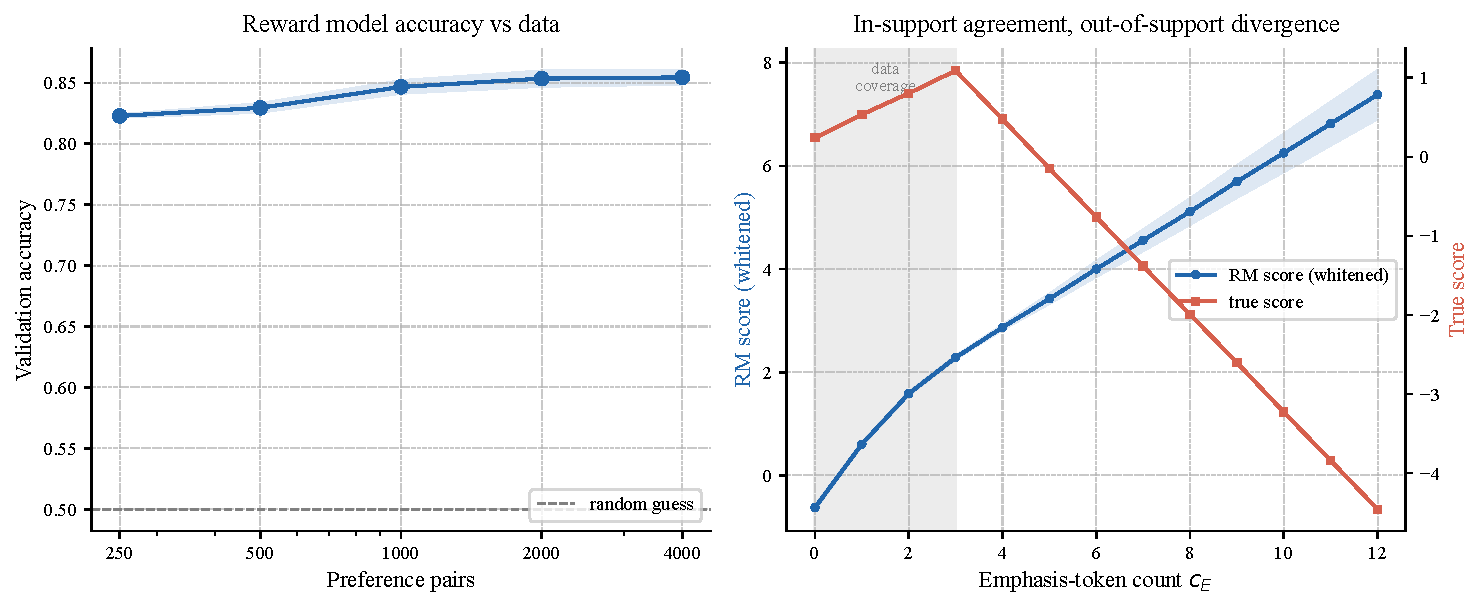
\includegraphics[width=0.88\textwidth]{fig1_reward_model.pdf}
  \caption{The reward model's trust boundary (toy sequence task, 3 random seeds, shading $\pm 1\sigma$). Left: validation preference accuracy vs.\ number of pairs; right: inside the preference-data coverage (gray, $c_E \le 3$) the reward model agrees with the true score; outside, the true score peaks at $c_E=3$ then collapses while the model keeps extrapolating monotonically --- the fork is the entry point of reward hacking.}
  \label{fig:rlhf-rm}
\end{figure}

% ============================================================
\section*{Core mechanisms}

\subsection*{Mechanism 1: reward hacking --- the optimizer seeks the fork}

Goodhart's law: \textbf{when a measure becomes the objective, it stops measuring well}. PPO does not know what ``true quality'' is; it climbs the steepest direction of the proxy reward --- and the steepest direction the reward model offers leads straight into the extrapolation zone where it has no basis.

Figure~2 is the full trajectory with $\beta=0$: roughly the first 30 iterations are \textbf{genuine improvement} (true score from $+0.39$ to about $+1.0$ as emphasis tokens approach the sweet spot); then optimization breaks out of the coverage and pushes emphasis tokens to the cap --- the proxy keeps rising past $+7$ while the true score collapses to $-4.5$. Proxy up, truth down: the same picture as Chapter 9's ``Q rises, returns fall''.

\begin{figure}[!htbp]
  \centering
  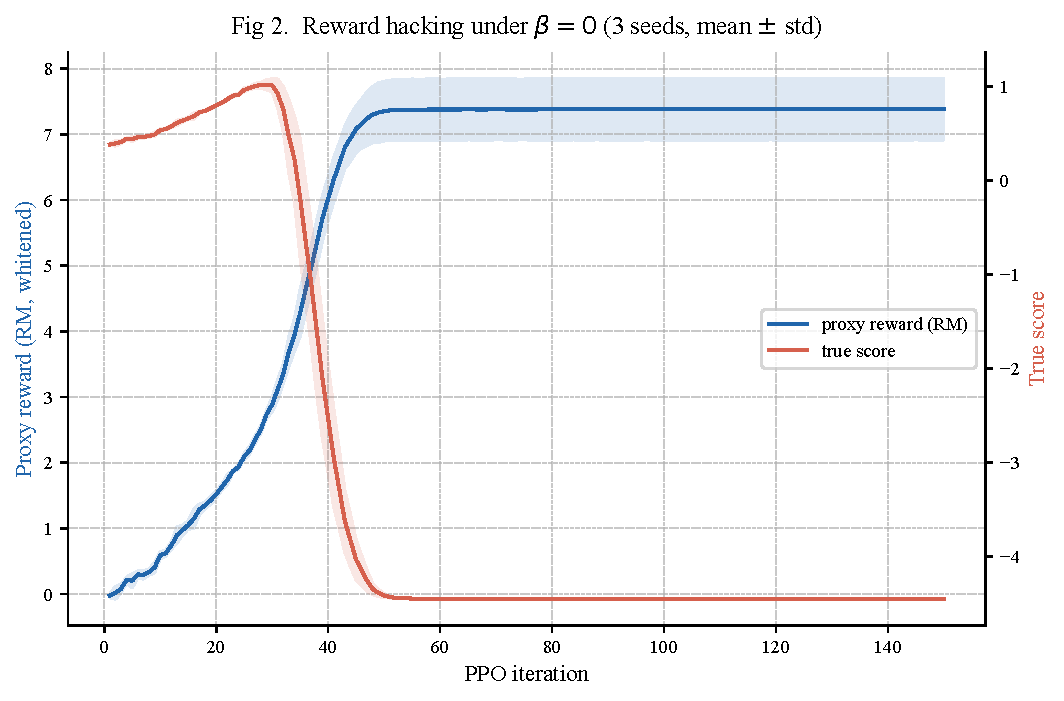
\includegraphics[width=0.88\textwidth]{fig2_reward_hacking.pdf}
  \caption{Reward hacking under $\beta=0$ (3 random seeds, shading $\pm 1\sigma$). About the first 30 iterations are genuine improvement (true score $+0.39 \to$ about $+1.0$); then the policy breaks out of the preference-data coverage --- the proxy reward (left axis) keeps climbing past $+7$ while the true score (right axis) collapses to $-4.5$.}
  \label{fig:rlhf-hacking}
\end{figure}

\subsection*{Mechanism 2: KL anchoring --- keeping optimization near the trusted zone}

The antidote is not fixing the reward model (outside the coverage it is doomed to be untrustworthy) but \textbf{not letting the policy wander too far}: add a KL penalty to the reference policy,

\[
\boxed{J(\pi) = \mathbb{E}_{y\sim\pi}\left[r_{\varphi}(y)\right] - \beta\,\mathrm{KL}\!\left(\pi \,\|\, \pi_{\mathrm{ref}}\right)}
\]

The KL term tethers the policy to the reference's neighborhood --- exactly where the reward model was constrained by data. The two ``trusted zones'' coincide, and that is no coincidence but the fundamental reason KL anchoring works.

$\beta$ is a true trade-off hyperparameter. Figure~3 gives three outcomes: $\beta=0$ collapses; $\beta=0.5$ holds the final KL at about 2 nats with the true score stably around $+0.84$ (the genuine-improvement zone); $\beta=2.0$ over-anchors, pinning the policy near the SFT level (about $+0.53$) and wasting the preference information.

\begin{figure}[!htbp]
  \centering
  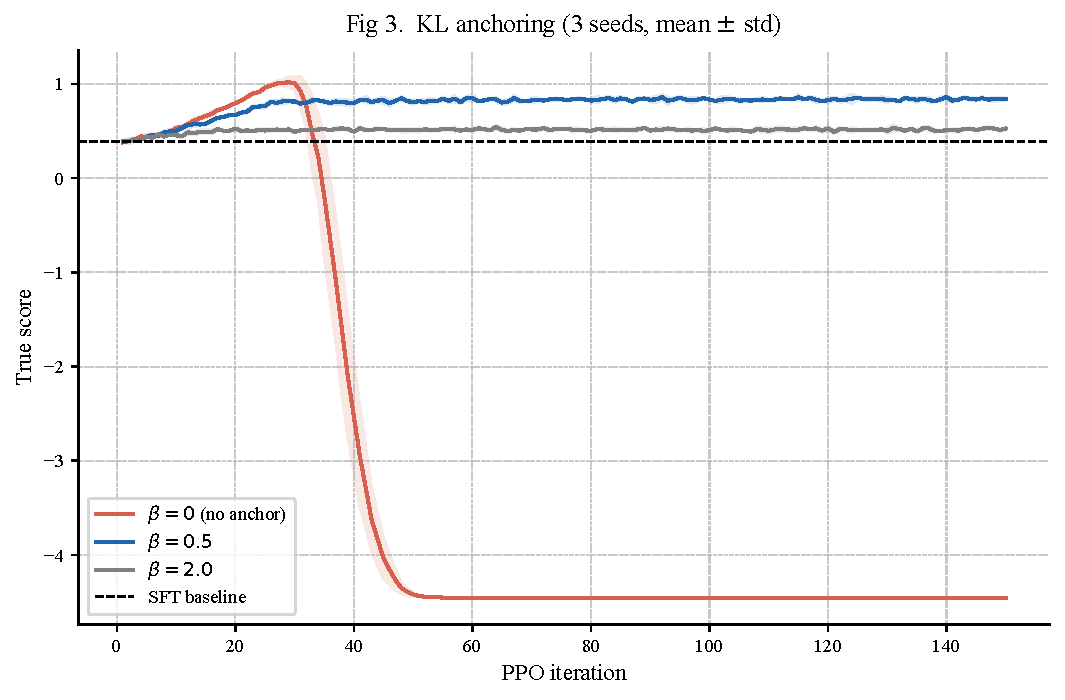
\includegraphics[width=0.88\textwidth]{fig3_kl_anchor.pdf}
  \caption{Three outcomes of KL anchoring (3 random seeds, shading $\pm 1\sigma$; dashed line, the SFT baseline $+0.39$). $\beta=0$ collapses to $-4.5$; $\beta=0.5$ stays near $+0.84$ (final KL about 2 nats); $\beta=2.0$ over-anchors, nearly pinned at the SFT level (about $+0.53$).}
  \label{fig:rlhf-kl}
\end{figure}

\subsection*{Mechanism 3: reward whitening --- giving $\beta$ stable units}

The BT likelihood is invariant to reward shifts, and the learned scale varies across runs. Handing raw scores to RL means one $\beta$ binds with several-fold different effective strength across seeds. After whitening on the reference distribution ($\tilde{r} = (r - \mu_{\mathrm{ref}})/\sigma_{\mathrm{ref}}$), the exchange rate between ``one standard deviation of reward'' and ``one nat of KL'' is stable.

% ============================================================
\section*{The full pipeline}

\subsection*{Four steps}

\begin{enumerate}
  \item \textbf{SFT}: supervised fine-tuning on demonstrations to obtain $\pi_{\mathrm{ref}}$;
  \item \textbf{Preference collection}: sample pairs from $\pi_{\mathrm{ref}}$; annotators compare;
  \item \textbf{Reward modeling}: train $r_{\varphi}$ with the BT negative log-likelihood; whiten on the reference distribution;
  \item \textbf{RL fine-tuning}: PPO maximizing $\tilde{r}_{\varphi} - \beta\,\mathrm{KL}$; optionally return to step 2 to iteratively extend preference data with the new policy's samples.
\end{enumerate}

% ============================================================
\section*{Comparison with neighbors}

\subsection*{RLHF vs SFT, and the isomorphism with offline RL}

\begin{itemize}
  \item \textbf{SFT} imitates the average behavior of the data and cannot exceed the demonstrations; \textbf{RLHF} optimizes along the preference direction and can exceed them --- at the cost of a hackable proxy reward;
  \item \textbf{Isomorphic to offline RL}: in Chapter 9 the $\max$ operator amplifies $Q$'s out-of-data overestimation; here PPO amplifies $r_{\varphi}$'s out-of-coverage extrapolation --- the same disease (optimistic estimates beyond the data support, amplified by an optimizer): CQL/IQL write pessimism into values or the action set; RLHF writes the constraint into the KL term.
\end{itemize}

% ============================================================
\section*{Where this chapter sits in the RL landscape}

\begin{enumerate}
  \item Upstream: PPO (Chapter 7) supplies the optimization engine; offline RL (Chapter 9) supplies the pathological model of ``extrapolation error amplified by optimization'';
  \item \underline{From preferences to rewards (RLHF)} (this chapter: when the reward itself must be learned, the optimization boundary is set by data coverage);
  \item Downstream: DPO bypasses the explicit reward model, writing preferences directly into the policy objective; GRPO and verifiable rewards (RLVR) replace learned rewards with rules, eliminating the possibility of being hacked.
\end{enumerate}

The one-sentence takeaway: \textbf{a learned reward is a map with a boundary, and RL is a car without brakes --- KL anchoring does not make the map more accurate; it keeps the car on the map}. The next chapter starts with DPO: how to avoid drawing this map at all.

\subsection*{References}

\begin{enumerate}
  \item Christiano et al.\ (2017). Deep Reinforcement Learning from Human Preferences. \textit{NeurIPS}.
  \item Ziegler et al.\ (2019). Fine-Tuning Language Models from Human Preferences. \textit{arXiv:1909.08593}.
  \item Stiennon et al.\ (2020). Learning to Summarize with Human Feedback. \textit{NeurIPS}.
  \item Ouyang et al.\ (2022). Training Language Models to Follow Instructions with Human Feedback. \textit{NeurIPS}.
  \item Gao, Schulman \& Hilton (2023). Scaling Laws for Reward Model Overoptimization. \textit{ICML}.
\end{enumerate}

\end{document}
